%%%%%%%%%%%%%%%%%%%%%%%%%%%%%%%%%%%%%%%%%%%%%%%%%%%%%%%%%%%%%%%%%%%%%%
%
% Numerical Methods for CSE, ETH Zuerich
%
% (C) Seminar for Applied Mathematics, D-MATH
%
%%%%%%%%%%%%%%%%%%%%%%%%%%%%%%%%%%%%%%%%%%%%%%%%%%%%%%%%%%%%%%%%%%%%%%
\documentclass[12pt]{report}
% Specific information for course
\newcommand{\lectyear}{2015}
\newcommand{\lectterm}{AT'15}
\newcommand{\lecturer}{Prof. Ralf Hiptmair}
\newcommand{\lecture}{NumCSE}

%\providecommand{\slidemode}{4}
\usepackage{samlecturenotes}

%%%%%%%%%%%%%%%%%%%%%%%%%%%%%%%%%%%%%%%%%%%%%%%%%%%%%%%%%%%%%%%%%%%%%%
% Version with Python programs (created by F. Thaler, AS 2015)
% MATLAB programs ported to Python and included in lecture document.
% Inclusion of python specific parts controlled by boolean switch
\newboolean{withpython}
\setboolean{withpython}{true}
%%%%%%%%%%%%%%%%%%%%%%%%%%%%%%%%%%%%%%%%%%%%%%%%%%%%%%%%%%%%%%%%%%%%%%

% symbol for external links
\newcommand{\ExternalLinkSymb}{
    \tikz[x=1.2ex, y=1.2ex, baseline=-0.05ex]{% 
        \begin{scope}[x=1ex, y=1ex]
            \clip (-0.1,-0.1) 
                --++ (-0, 1.2) 
                --++ (0.6, 0) 
                --++ (0, -0.6) 
                --++ (0.6, 0) 
                --++ (0, -1);
            \path[draw, 
                line width = 0.5, 
                rounded corners=0.5] 
                (0,0) rectangle (1,1);
        \end{scope}
        \path[draw, line width = 0.5] (0.5, 0.5) 
            -- (1, 1);
        \path[draw, line width = 0.5] (0.6, 1) 
            -- (1, 1) -- (1, 0.6);
        }
    }

% Graphics input path
\graphicspath{
{./Images/}
{./PICS/}
{./p1_SystemsOfEquations/Triangulations/}
{./p1_SystemsOfEquations/ch1_MatVec/PICTURES/}
{./p1_SystemsOfEquations/ch2_DirectMethodsLSE/PICTURES/}
{./p1_SystemsOfEquations/ch3_IterativeMethodsNonLinear/PICTURES/}
{./p1_SystemsOfEquations/ch4_IterativeMethodsLSE/PICTURES/}
{./p1_SystemsOfEquations/ch5_Eigenvalues/PICTURES/}
{./p1_SystemsOfEquations/ch6_LeastSquares/PICTURES/}
{./p1_SystemsOfEquations/ch7_Convolution/PICTURES/}
{./p1_SystemsOfEquations/ch8_FFT/PICTURES/}
{./p2_InterpolationApproximation/ch1_PolynomialInterpolation/PICTURES/}
{./p2_InterpolationApproximation/ch2_PiecewisePolynomials/PICTURES/}
{./p2_InterpolationApproximation/ch4_NumericalQuadrature/PICTURES/}
{./p2_InterpolationApproximation/ch6_ClusteringTechniques/PICTURES/}
{./p2_InterpolationApproximation/ch3_TrigonometricInterpolation/PICTURES/}
{./p2_InterpolationApproximation/ch5_FilteringWavelets/PICTURES/}
{./p3_ODE/ch1_SingleStepMethods/PICTURES/}
{./p3_ODE/ch2_ConvergenceStability/PICTURES/}
{./Maturandentag/PICTURES/}
}

\externaldocument{./NCSENEW}

%%%%%%%%%%%%%%%%%%%%%%%%%%%%%%%%%%%%%%%%%%%%%%%%%%%%%%%%%%%%
% Include macros
%%%%%%%%%%%%%%%%%%%%%%%%%%%%%%%%%%%%%%%%%%%%%%%%%%%%%%%%%%%%
\input{NCSENEW_macros}

% Partial compilation when in editing mode (selective inclusion)
%\ifthenelse{\equal{4}{\slidemode}}
%{%
%  \includeonly{NCSENEW_Testproblem}{}
%}{}

% Import SVN revision

\newcounter{svnrevision}\setcounter{svnrevision}{
 84575}


\begin{document}

\begin{tcolorbox}[colframe=black]
\begin{minipage}[t][0.6\textwidth][c]{\textwidth}
  ETH Lecture 401-0663-00L  Numerical Methods for CSE 
  \B\vspace{1.5cm}
  
  \begin{center}
    \Red{\Huge Homework Problems}
  \end{center}
  \vspace{1.5cm}
  
  \begin{center}
  \begin{large}
    {\Large Prof. R. Hiptmair, SAM, ETH Zurich}\\[1.5ex]

    Autumn Term 2016 %  draft version \svnToday, SVN rev. \svnInfoRevision

    (C) Seminar f\"ur Angewandte Mathematik, ETH Z\"urich
    \samskip

    URL: \href{http://www.sam.math.ethz.ch/~hiptmair/tmp/NumCSE/NumCSE15.pdf}{%
      http://www.sam.math.ethz.ch/\symbol{126}hiptmair/tmp/NumCSE/NumCSE15.pdf}
  \end{large}
\end{center}
\end{minipage}
\end{tcolorbox}
\bigskip

%%%%%%%%%%%%%%%%%%%%%%%%%%%%%%%%%%%%%%%%%%%%%%%%%%%%%%%%%%%%
% General information
%%%%%%%%%%%%%%%%%%%%%%%%%%%%%%%%%%%%%%%%%%%%%%%%%%%%%%%%%%%%
\fboxsep1ex
\fbox{\parbox{0.95\textwidth}{
    A steady and persistent effort spent on homework problems is essential for
    success in the course.
}}
\bigskip

You should expect to spend 4-6 hours per week on trying to solve the homework
problems. Since many involve small coding projects, the time it will take an
individual student to arrive at a solution is hard to predict.  
\bigskip

\begin{itemize}
\item The assignment sheets will be uploaded on the course
  \href{http://www2.math.ethz.ch/education/bachelor/lectures/hs2015/math/nummath_cse/index}{webpage}
  on Thursday every week.
\item Some or all of the problems of an assignment sheet will be discussed in the
  tutorial classes on Monday 1$\frac{1}{2}$ weeks after the problem sheet has been
  published.
\item A few problems on each sheet will be marked as {\bf core problems}. 
  Every participant of the course is strongly advised to try and solve \emph{at least}
  the core problems. 
\item If you want your tutor to examine your solution of the current problem
  sheet, please put it into the plexiglass trays in front of HG G 53/54 by the
  Thursday after the publication. You should submit your codes using the
  \href{https://people.math.ethz.ch/~grsam/submit/}{online submission
    interface}. This is voluntary, but feedback on your performance on homework
  problems can be important.
\item You are encouraged to hand-in incomplete and wrong solutions, since 
  you can receive valuable feedback even on incomplete attempts.
\item Please clearly mark the homework problems that you want your tutor to
  examine.
\end{itemize}

%%%%%%%%%%%%%%%%%%%%%%%%%%%%%%%%%%%%%%%%%%%%%%%%%%%%%%%%%%%%
% Selective inclusion of Problems
%%%%%%%%%%%%%%%%%%%%%%%%%%%%%%%%%%%%%%%%%%%%%%%%%%%%%%%%%%%%

%\chapter{Matrix Vector}
\Label{cha:matvec}

\begin{samproblem}*{prb:gramschmidteigen}{Gram-Schmidt orthogonalization with \eigen{}}[1]{
\cref{gramschmidt} presents a \matlab{} code that effects the Gram-Schmidt
  orthogonalization of the columns of an argument matrix. 
}

\begin{subproblem}{sp:1}[1]
  Based on the C++ linear algebra library \eigen{} implement a function

  \begin{samcode}[C++-code]{cpp:signature}{Function prototype}
    \begin{lstlisting}[style=cpp]
template <class Matrix>  
Matrix gramschmidt(const Matrix &A);
    \end{lstlisting}
  \end{samcode}
  that performs the same computations as \cref{gramschmidt}. 

  \begin{samhint}
    Use \eigen{}s block operations (see \href{https://eigen.tuxfamily.org/dox/group__TutorialBlockOperations.html}{\ExternalLinkSymb})
  \end{samhint}

  % BEGIN ================ SOLUTION  ================   %
  \begin{samsolution}
    \begin{samcode}[C++-code]{\cpl:cpp:solution}{Gram-Schmidt orthogonalization with \eigen{}}
      \lstinputlisting[style=cpp_problem]{../Solutions/MatVec/gramschmidt/gramschmidt.hpp}
    \end{samcode}
  \end{samsolution}
  % END ================ SOLUTION  ================   %

\end{subproblem}

\begin{subproblem}{sp:2}[1]
  \label{sp:strassen:2}
  Test your implementation by applying it to a small random matrix
  and checking the orthonormality of the columns of the output
  matrix.

  % BEGIN ================ SOLUTION  ================   %
  \begin{samsolution}
    \begin{samcode}[C++-code]{\cpl:cpp:solution}{Gram-Schmidt orthogonalization with \eigen{}}
      \lstincludecpp[style=cpp_problem]{../Solutions/MatVec/gramschmidt/main.cpp}{1}
    \end{samcode}
  \end{samsolution}
  % END ================ SOLUTION  ================   %

\end{subproblem}

\end{samproblem}



%\begin{samproblem}*{prb:fastmatmult}{Fast matrix multiplication with \eigen{}}[1]{
\cref{rem:strassen} presents Strassen's algorithm that can achieve
  the multiplication of two dense square matrices of size {$n=2^{k}$},
  $k\in\bbN$, with an asymptotic complexity better than $O(n^{3})$.
}

\begin{subproblem}{sp:1}[1]
	Using \eigen~ implement a function
	\begin{lstlisting}[style=cppsimple]
	 MatrixXd strassenMatMult(const MatrixXd & A, const MatrixXd & B)
	\end{lstlisting}
	that uses Strassen's algorithm to multiply the two matrices $\VA$ and
	$\VB$ and return the result as output. 

  % BEGIN ================ SOLUTION  ================   %
  \begin{samsolution}
    \begin{samcode}[C++-code]{\cpl:cpp:solution}{Strassen's algorithm with \eigen{}}
      \lstincludecpp[style=cpp_problem]{../Solutions/MatVec/fastmatmult/strassen.cpp}{1}
    \end{samcode}
  \end{samsolution}
  % END ================ SOLUTION  ================   %

\end{subproblem}

\begin{subproblem}{sp:2}[1]
	Validate the correctness of your code by comparing the result
    with \eigen's built-in matrix multiplication.

  \begin{samsolution}
    \begin{samcode}[C++-code]{\cpl:cpp:solution}{Strassen's algorithm with \eigen{}}
      \lstincludecpp[style=cpp_problem]{../Solutions/MatVec/fastmatmult/strassen.cpp}{1}
    \end{samcode}
  \end{samsolution}
\end{subproblem}

\begin{subproblem}{sp:3}[1]
	Measure the runtime of your function
    \lstinline[style=cppsimple]|strassenMatMult|
    for random matrices of sizes $2^{k}$, $k=4,\ldots,10$, and compare
    with the matrix multiplication offered by the $\ast$-operator
    of \eigen{}.

  \begin{samhint}
    Use the optimization capabilities of your C++ compiler by appending \\ \lstinline[style=cppsimple]|-DCMAKE_BUILD_TYPE=RELEASE| to the cmake invocation in order to get reliable timings. Please note that this also disables various integrity checks.
  \end{samhint}
  \begin{samhint}
    Ensure that the compiler does not optimize away your computation by using the result of the multiplication in some fashion (e.g. by summing one coefficient of the result matrix and printing it after all measurements finished).
  \end{samhint}
\end{subproblem}

\end{samproblem}

\chapter{Matrix Vector}
\Label{cha:matvec}

%%%%%%%%%%%%%%%%%%%%%%%%%%%%%%%%%%%%%%%%%%%%%%
% Test problem for new environment 'samproblem'
%%%%%%%%%%%%%%%%%%%%%%%%%%%%%%%%%%%%%%%%%%%%%%

\begin{samproblem}*{prb:gramschmidteigen}{Gram-Schmidt orthogonalization with \eigen{}}[1]{
\cref{gramschmidt} presents a \matlab{} code that effects the Gram-Schmidt
  orthogonalization of the columns of an argument matrix. 
}

\begin{subproblem}{sp:1}[1]
  Based on the C++ linear algebra library \eigen{} implement a function

	\begin{samcode}[C++-code]{cpp:signature}{Function prototype}
		\begin{lstlisting}[style=cpp]
template <class Matrix>  
Matrix gramschmidt(const Matrix &A);
		\end{lstlisting}
	\end{samcode}
	that performs the same computations as \cref{gramschmidt}. 


  % BEGIN ================ SOLUTION  ================   %
  \begin{samwriteprbpart}{testsol}
    \begin{writeverbatim}{prbfile}
      \begin{samsolution}
				\begin{samcode}[C++-code]{\cpl:cpp:solution}{Gram-Schmidt orthogonalization with \eigen{}}
					\lstinputlisting[style=cpp]{Chapters/MatrixVector/CPP/gramschmidt.cpp}
				\end{samcode}
      \end{samsolution}
    \end{writeverbatim}
  \end{samwriteprbpart}
  % END ================ SOLUTION  ================   %

\end{subproblem}

\begin{subproblem}{sp:2}[1]
	\label{sp:strassen:2}
	Test your implementation by applying it to a small random matrix
	and checking the orthonormality of the columns of the output
	matrix.

  % BEGIN ================ SOLUTION  ================   %
  \begin{samwriteprbpart}{testsol}
    \begin{writeverbatim}{prbfile}
      \begin{samsolution}
				See \prbref{cpp:solution}
      \end{samsolution}
    \end{writeverbatim}
  \end{samwriteprbpart}
  % END ================ SOLUTION  ================   %

\end{subproblem}

\end{samproblem}




% ncse_new/p1_SystemsOfEquations/ch1_MatVec/ex_ArrowMatrixVector.tex
% the exercise requires:    arrowmatvec.m    arrowmatvectiming.eps    arrowmatvectiming.jpg
% the solutions require:    arrowmatvec2.m    arrowmatvec2timing.m    arrowmatvec2timing.eps

\begin{samproblem}{prb:ArrowMatrixVector}{Arrow matrix-vector multiplication (core problem)}{
Consider the multiplication of the two ``arrow matrices'' $\VA$ with a vector $\Vx$,
implemented as a function \texttt{arrowmatvec(d,a,x,y)} in \cref{cpp:arrowmatvec}
}
\begin{samcode}[C++-code]{cpp:arrowmatvec}{multiplying a vector with the product of two ``arrow matrices''}
  \lstinputlisting[style=cpp]{Chapters/MatrixVector/CPP/arrowmatvec.hpp}
\end{samcode}

\begin{samhint}
This \cpp~ code is provided as file \texttt{arrowmatvec.hpp}.
\end{samhint}

%%%%%%%%%%%% SUBPROBLEM 1

\begin{subproblem}{sp:1}[1]
  For general vectors $d = (d_1, \dots, d_n)^\top$ and $a = (a_1, \dots, a_n)^\top$, sketch the matrix $\VA$ created in \autoref{cpp:arrowmatvec}.

  % BEGIN ================ SOLUTION  ================   %
  \begin{samwriteprbpart}{solfile}
    \begin{writeverbatim}{prbfile}
      \begin{samsolution}
        $\VA=\begin{pmatrix}
         d_1 &     &        &         &  a_1     \\
             & d_2 &        &         &  a_2     \\
             &     & \ddots &         &  \vdots  \\
             &     &        & d_{n-1} &  a_{n-1} \\
         a_1 & a_2 & \dots  & a_{n-1} &  d_n     \\
        \end{pmatrix}$
      \end{samsolution}
    \end{writeverbatim}
  \end{samwriteprbpart}
  % END ================== SOLUTION  ================   %
\end{subproblem}

%%%%%%%%%%%% SUBPROBLEM 2

\begin{subproblem}{sp:2}[2]
  The timing results for \texttt{arrowmatvec.cpp} are available in \autoref{fig:arrowmatvectiming}. 
  Give a detailed explanation of the results.

  \begin{figure}[ht]
    \centering
    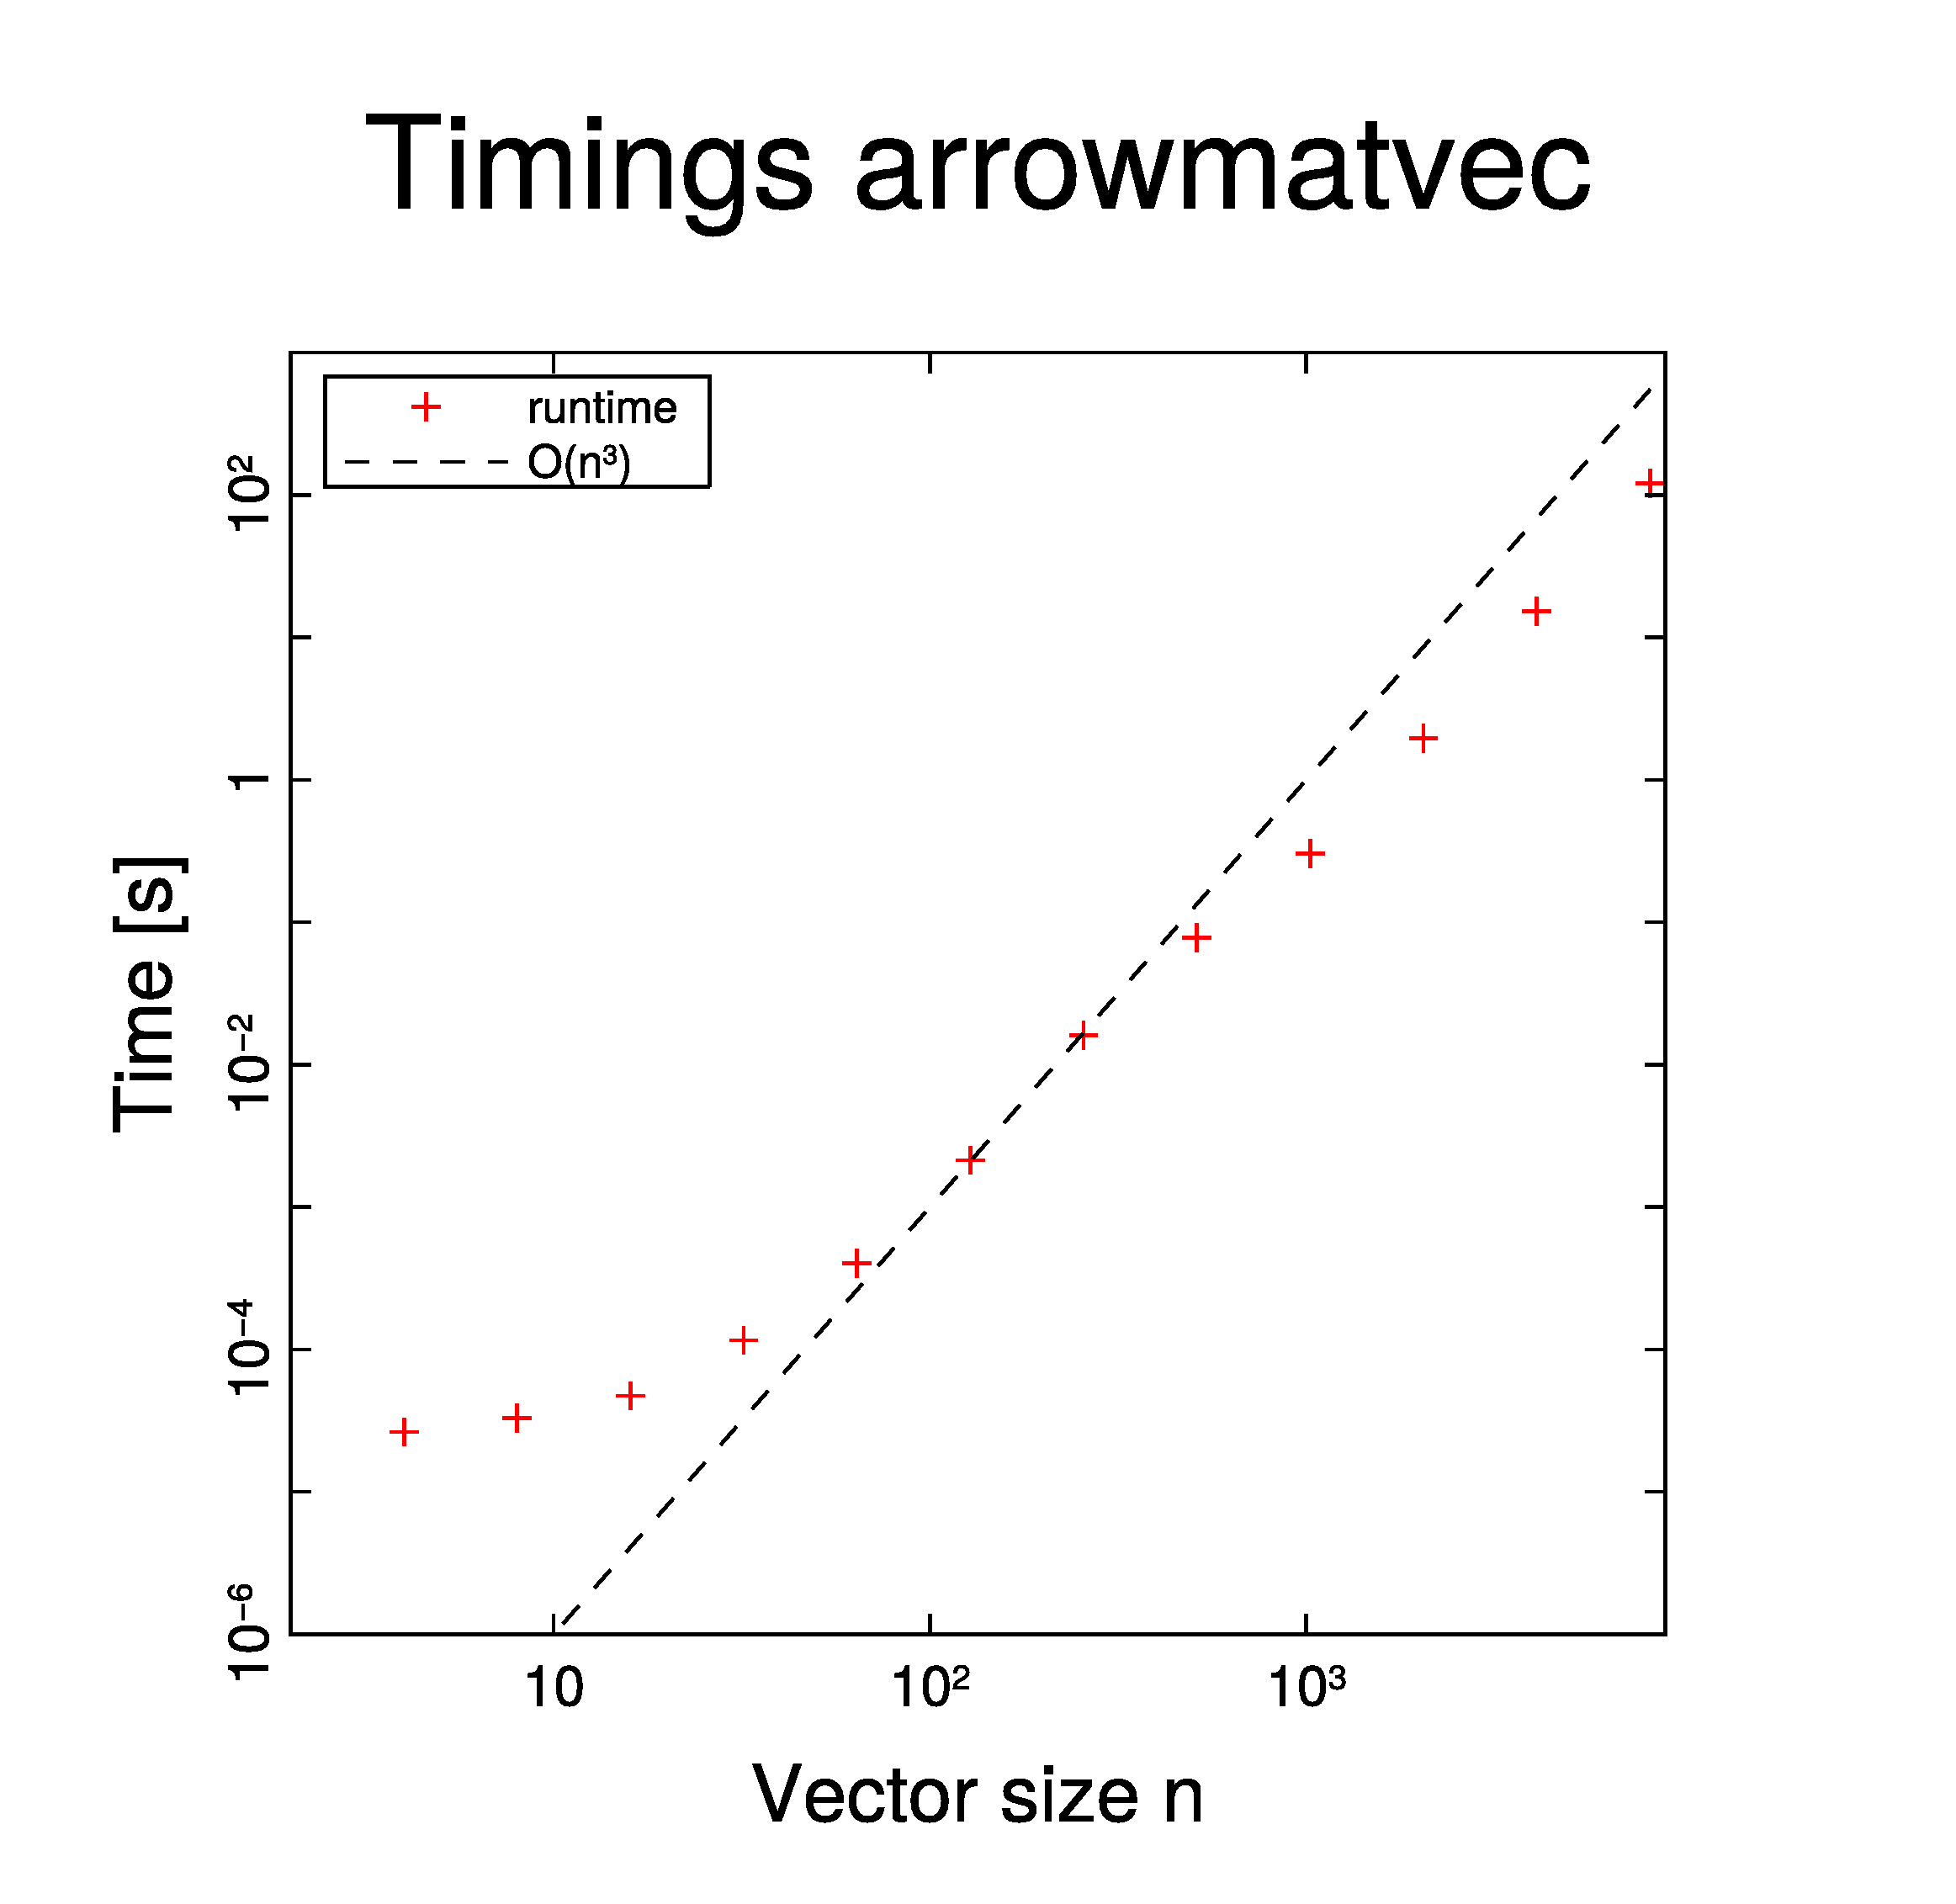
\includegraphics[width=0.8\textwidth]{Chapters/MatrixVector/PICTURES/arrowmatvectiming.eps}
    \caption{timings for \texttt{arrowmatvec(d,a,x)}}
    \label{fig:arrowmatvectiming}
  \end{figure}

  \begin{hint}
    This \cpp~ created figure is provided as file
    \texttt{arrowmatvectiming.\{eps,jpg\}}.
  \end{hint}

  % BEGIN ================ SOLUTION  ================   %
  \begin{samwriteprbpart}{solfile}
    \begin{writeverbatim}{prbfile}
      \begin{samsolution}
      The standard matrix-matrix multiplication has runtimes growing with $O(n^3)$ 
      and the standard matrix-vector multiplication has runtimes growing with $O(n^2)$. 
      Hence, the overall computational complexity is dominated by $O(n^3)$.
      \end{samsolution}
    \end{writeverbatim}
  \end{samwriteprbpart}
  % END ================== SOLUTION  ================   %
\end{subproblem}

%%%%%%%%%%%% SUBPROBLEM 3
\begin{subproblem}{sp:3}[3]
  Write an \emph{efficient} \cpp~ function 
  \begin{samcode}[C++-code]{cpp:sp3}{Function prototype}
    \begin{lstlisting}[style=cpp]
template <class Matrix>
void arrowmatvec2(const Matrix& d, const Matrix& a, const Matrix& x, Matrix& y)
    \end{lstlisting}
  \end{samcode}
  that computes the same multiplication as in code \ref{cpp:arrowmatvec} but with optimal asymptotic complexity with respect to {$n$}.
  Here \texttt{d} passes the vector $(d_{1},\ldots,d_{n})^{T}$ and \texttt{a} passes the vector $(a_{1},\ldots,a_{n})^{T}$.

  % BEGIN ================ SOLUTION  ================   %
  \begin{samwriteprbpart}{solfile}
    \begin{writeverbatim}{prbfile}
      \begin{samsolution}
      Due to the sparsity and special structure of the matrix, it is possible to write a more efficient implementation than the standard matrix-vector multiplication. 
      See code listing \ref{cpp:arrowmatvec2}

      \begin{samcode}[C++-code]{cpp:arrowmatvec2}{implementation of the function \texttt{arrowmatvec2}}
        \lstinputlisting[style=cpp]
        {Chapters/MatrixVector/CPP/arrowmatvec2.hpp}
      \end{samcode}

      \end{samsolution}
    \end{writeverbatim}
  \end{samwriteprbpart}
  % END ================== SOLUTION  ================   %

\end{subproblem}
%%%%%%%%%%%% SUBPROBLEM 4

\begin{subproblem}{sp:4}[1]
  What is the complexity of your algorithm from sub-problem \ref{sp:3} (with respect to problem size $n$)? 

  % BEGIN ================ SOLUTION  ================   %
  \begin{samwriteprbpart}{solfile}
    \begin{writeverbatim}{prbfile}
      \begin{samsolution}
      The efficient implementation only needs two vector-vector element-wise multiplications and one vector-scalar multiplication. 
      Therefore the complexity is $O(n)$.
      \end{samsolution}
    \end{writeverbatim}
  \end{samwriteprbpart}
  % END ================== SOLUTION  ================   %

\end{subproblem}

%%%%%%%%%%%% SUBPROBLEM 5

\begin{subproblem}{sp:5}[2]
  Compare the runtime of your implementation and the implementation given in code \ref{cpp:arrowmatvec} for $n=2^{5,6,\ldots,12}$.
  Use the \texttt{std::chrono} package (see \hyperlink{link}{\Blue{here}}) or use the provided library \texttt{timer.h}.

  % BEGIN ================ SOLUTION  ================   %
  \begin{samwriteprbpart}{solfile}
    \begin{writeverbatim}{prbfile}
      \begin{samsolution}
      The standard matrix multiplication has runtimes growing with $O(n^3)$.
      The runtimes of the more efficient implementation are growing with $O(n)$.
      See \autoref{cpp:arrowmatvec2timing} and Figure~\ref{fig:arrowmatvec2timing}.

      \begin{samcode}[C++-code]{cpp:arrowmatvec2timing}{Execution and timings of \texttt{arrowmatvec} and \texttt{arrowmatvec2}}
        \lstinputlisting[style=cpp]
        {Chapters/MatrixVector/CPP/arrowmatvec2timing.cpp}
      \end{samcode}

      \begin{figure}[ht]
        \centering
        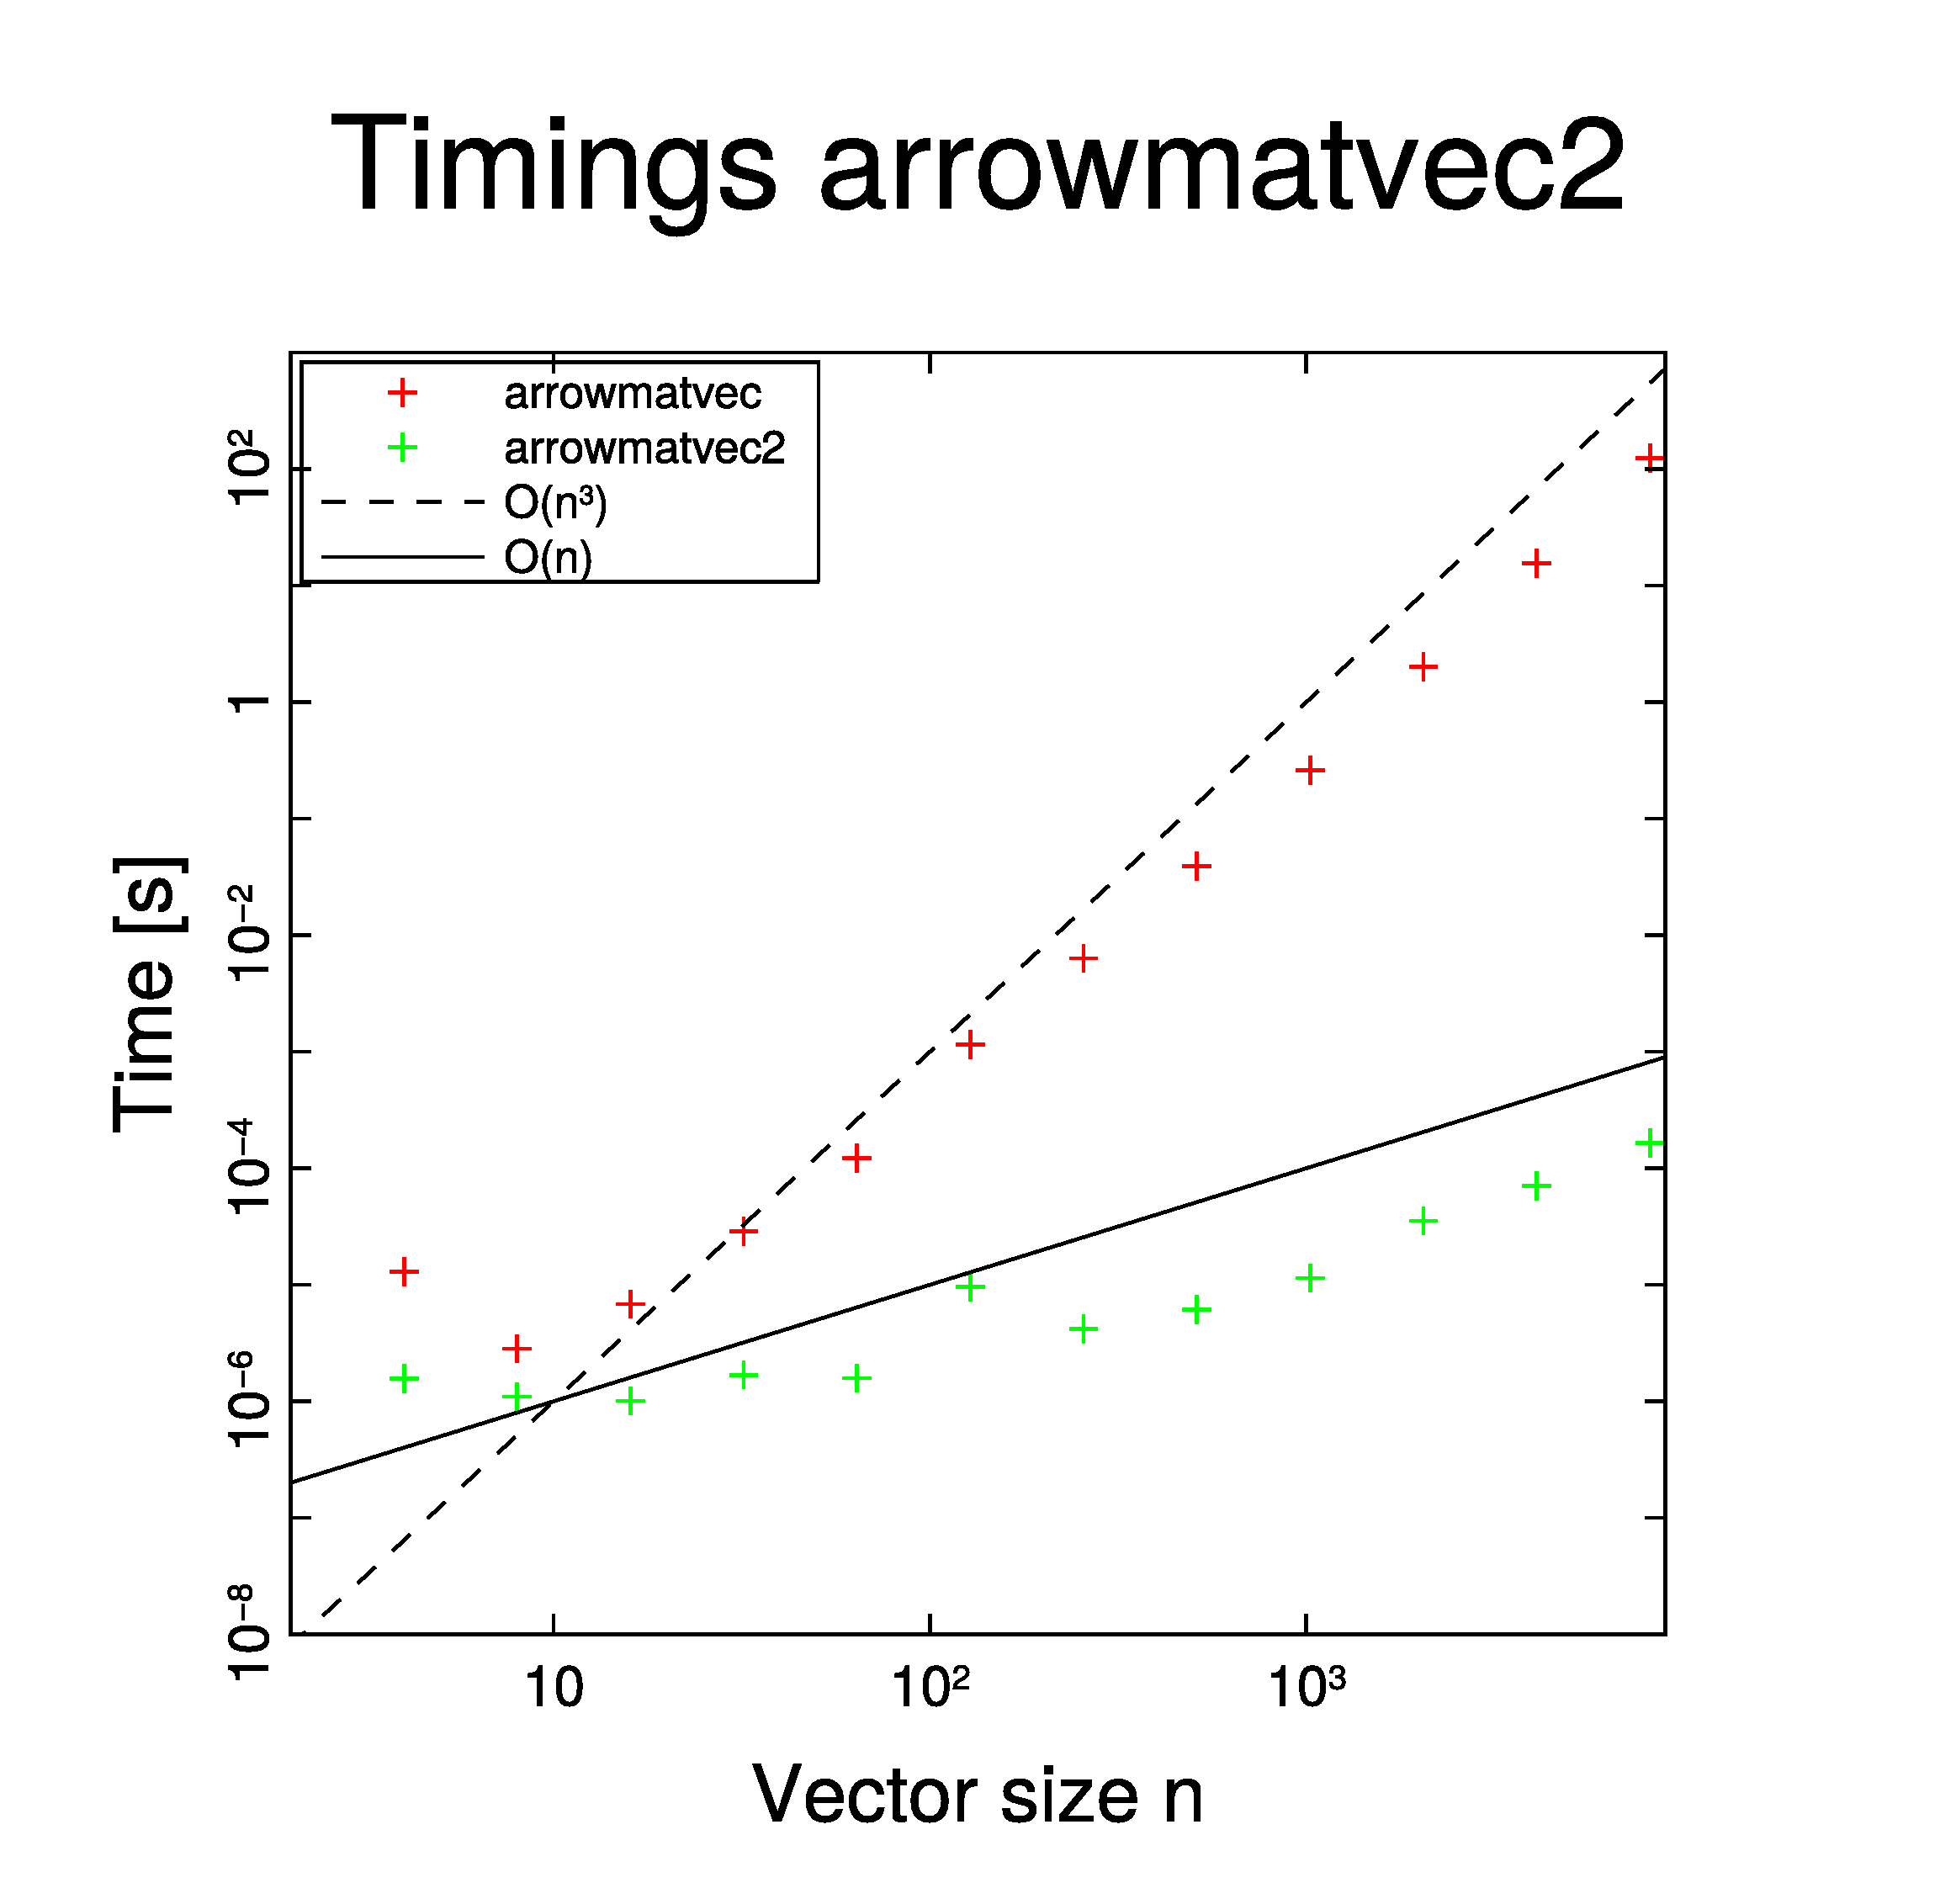
\includegraphics[width=0.8\textwidth]{Chapters/MatrixVector/PICTURES/arrowmatvec2timing.eps}
        \caption{timings for \texttt{arrowmatvec2(d,a,x,y)}} \label{fig:arrowmatvec2timing}
      \end{figure}
      \end{samsolution}
    \end{writeverbatim}
  \end{samwriteprbpart}
  % END ================== SOLUTION  ================   %

\end{subproblem}


%% this subproblem does only make sense if the other problems are using Matlab codes
%\begin{subproblem}[1] \label{subprb:ArrowMatrixVector_6}
%Write the \eigen{} codes corresponding to the functions \texttt{arrowmatvec} and \texttt{arrowmatvec2}.
%
%\begin{solution}
%See Listing~\ref{cppc:arrowmatvec} and Listing~\ref{cppc:arrowmatvec2}.
%
%\lstinputlisting[style=cpp,caption={Implementation of \texttt{arrowmatvec}  in \eigen{}},label={cppc:arrowmatvec}]
%{\problems/\chpt/CPP/arrowmatvec.cpp}
%
%\lstinputlisting[style=cpp,caption={Implementation of \texttt{arrowmatvec2}  in \eigen{}},label={cppc:arrowmatvec2}]
%{\problems/\chpt/CPP/arrowmatvec2.cpp}
%\end{solution}
%\end{subproblem}

\end{samproblem}


\chapter{Test Problems}
\Label{cha:prb}

%%%%%%%%%%%%%%%%%%%%%%%%%%%%%%%%%%%%%%%%%%%%%%
% Test problem for new environment 'samproblem'
%%%%%%%%%%%%%%%%%%%%%%%%%%%%%%%%%%%%%%%%%%%%%%

\begin{samproblem}*{prb:test}{Test problem}[3](15){This problem tests the new \texttt{samproblem} \LaTeX environment.

It is related to \cref{sec:cpp} and considers the following formula
\begin{sammath}{gather}
  \prblabel{eq:0}
  s = \sum\limits_{k=0}^{n}f(k)\;\bdot
 \end{sammath}%
}

\begin{samhint}
  This is a lonely hint at the toplevel of \cref{prb:test}. 
\end{samhint}

\begin{subproblem}{sp:1}[3](3)
  \par\begin{lstlisting}[style=cpp]
template <typename Function>
double proccess(Function &f,const std::vector<double> &x) {
  double s = 0;
  // Sum according to \prbeqref{eq:0}
  for(auto i : x) { s += f(i); } 
  return s; 
}
\end{lstlisting}

We consider the integral 
\begin{sammath}{gather}
  \prblabel{eq:1}
  \int\limits_{0}^{1}e^{x}\,\textrm{d}e = ?
\end{sammath}%
In \prbref{eq:1} we see the disturbing impact of alien notation, see also \cref{par:ops}.

  % BEGIN ================ OUTPUT  ================   %
  \begin{samwriteprbpart}{h1}
    \begin{writeverbatim}{prbfile}
      \begin{samhint}
        Recall \prbcref{eq:1}!
      \end{samhint}
    \end{writeverbatim}
  \end{samwriteprbpart}
  
  % BEGIN ================ OUTPUT  ================   %
  \begin{samwriteprbpart}{h2}
    \begin{writeverbatim}{prbfile}
      \begin{samhint}
        Take into account \cref{mc:sa3} and
        \begin{sammath}{gather}
          \prblabel{h:1}
          a^{2} - b^{2} = (a+b)(a-b)\;\bdot
        \end{sammath}%
      \end{samhint}
    \end{writeverbatim}
  \end{samwriteprbpart}

  % BEGIN ================ OUTPUT  ================   %
  \begin{samwriteprbpart}{testsol}
    \begin{writeverbatim}{prbfile}
      \begin{samsolution}
        We make use of \prbeqref{h:1} and \prbeqref{eq:1} and conclude
        \begin{sammath}{gather}
          \prblabel{s:1}
          1*1 = 1 !
        \end{sammath}%
      \end{samsolution}
    \end{writeverbatim}
  \end{samwriteprbpart}

\end{subproblem}

This is text between \prbcref{sp:1} and \prbcref{sp:2}. 

\begin{subproblem}{sp:2}<\prbref{sp:1}>
  This subproblem continues \prbcref{sp:1} and looks at
  \begin{sammath}{gather}
    \prblabel{eq:2}
    \btext{\prbeqref{eq:1}}\quad \Black{\Rightarrow}\quad
    x^{2} = x-1\;\bdot
  \end{sammath}%
  The entire sub-problem is indented. 

  
  % BEGIN ================ OUTPUT  ================   %
  \begin{samwriteprbpart}{sol}
    \begin{writeverbatim}{prbfile}
      \begin{samsolution}
        This is the solution of \prbcref{sp:2}!

        \begin{minipage}[c]{0.5\textwidth}
          This means
          \begin{sammath}{gather}
            \prblabel{pl:1}
            1 + 1 = 2 !
          \end{sammath}%
          and this might be related to \prbeqref{h:1}, see
          \cref{drawing}.
        \end{minipage}%
        \begin{minipage}[c]{0.5\textwidth}
          \samplot{drawing}
        \end{minipage}%
      \end{samsolution}
    \end{writeverbatim}
  \end{samwriteprbpart}
\end{subproblem}

\end{samproblem}

\bigskip 

Outside the problem we can reference equations: \eqref{prb:test:eq:0} or 
\cref{prb:test:eq:1}.

We can also referennce \cref{prb:test:sp:2} or \ref{prb:test:sp:2}.
\bigskip


%

\section{Inclusion of Codes}

Parts of a C++ code can be included by means of the \verb|\lstincludecpp| command:

Included with tag 2:

\begin{samcode}[C++ code]{cpp:1}{A demo code}
  \lstincludecpp[emph={NPDE},linebackgroundcolor={\lstcolorrange{2}{4}}]{test.cpp}{2}
\end{samcode}

Note \cref{l:1}! Included with tag 4, same file as \cref{cpp:1}.

\lstincludecpp[emph={Constant},linebackgroundcolor={\lstcolorlines{1,3,5}}]{test.cpp}{4}

\chapter{Summary}
\Label{cha:sum}

\cref{prb:test}: This is a test problem for demonstration only


\bibliographystyle{plain} 
\bibliography{lit}

\end{document}

